\section{Mechanical}
\label{sec:implementation-mechanical}

\begin{figure}[h]
	\centering
	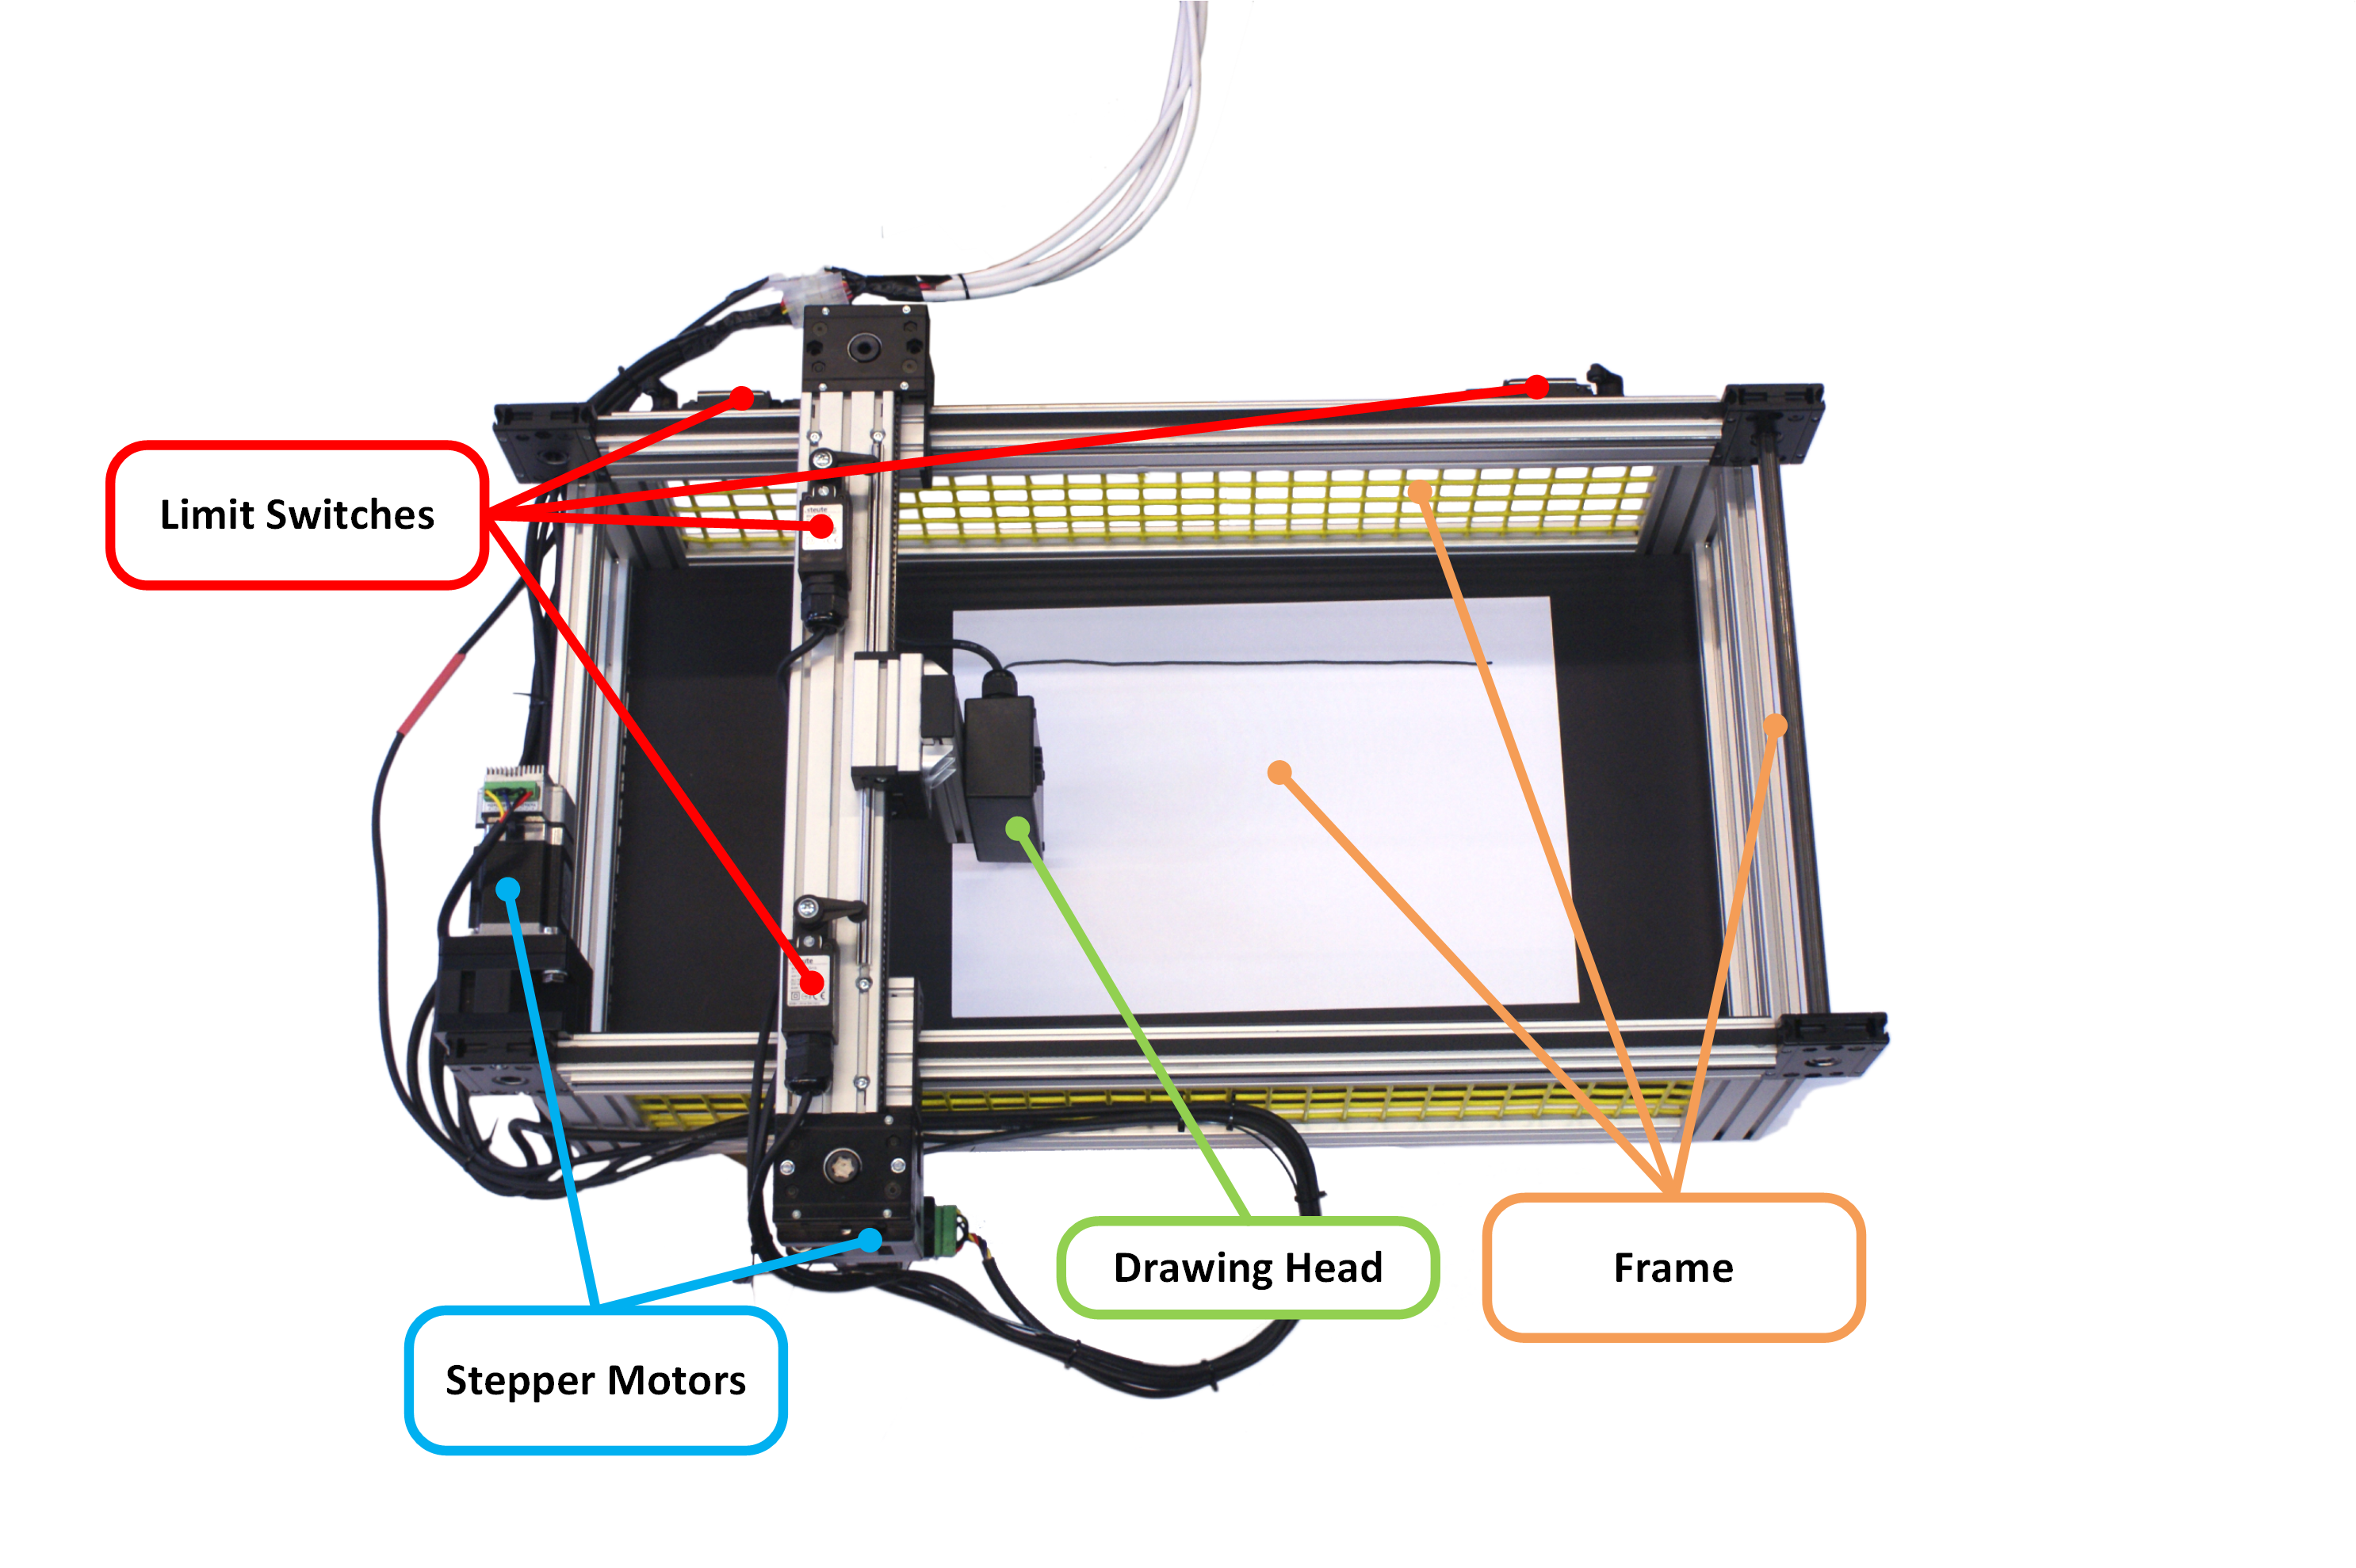
\includegraphics[trim=10mm 0mm 40mm 28mm, clip, width=0.75\textwidth]{figures/cncMachine/mechanical.png}
	\caption{The DoodleBot mechanical hardware}
	\label{fig:implementation-mechanical}
\end{figure}

\begin{table}
	\centering
	\begin{tabular}{|c|c|c|}
		\hline
		\emph{Parameter} & \emph{Size} & \emph{Units}\\ \hline
		Machine dimensions & 866x604x300 & mm (LxWxH)\\ \hline
		Drawing Area X & 560 & mm\\ \hline
		Drawing Area Y & 280 & mm\\ \hline
		X Frame Resolution & 140 & mm/revolution\\ \hline
		Y Frame Resolution & 140 & mm/revolution\\ \hline
		Motor resolution & 2000 & steps/revolution\\ \hline
		X Resolution & 0.007 & mm/step\\ \hline 
		Y Resolution & 0.007 & mm/step\\ \hline
	\end{tabular}
\end{table}

\subsection{Frame}
	The DoodleBot frame was procured by NHP and was a purpose built product made by Item America. It includes an extruded aluminium frame, with a direct (no gearing) belt-driven system. The frame is designed with mounts to match the stepper motors. 
\subsection{Motors}
	\begin{figure}[h]
		\centering
		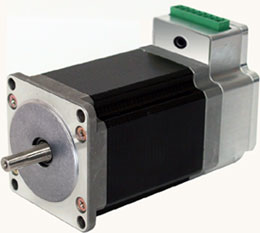
\includegraphics[width=0.2\textwidth]{figures/cncmachine/amci-smd23.jpg}
		\caption{An AMCI SMD23 stepper motor with integrated driver}
	\end{figure}
	
	The DoodleBot uses two AMCI SMD23 stepper motors with integrated drivers to drive the dynamics of the X and Y axes respectively. The SMD23 has an integrated driver which controls the activation of the internal stepper motor electromagnets and only needs to be provided with power, a step signal and a direction signal.
\subsection{Limit Switches}
	The limit switches are <model> and are mounted such that as either of the axes approach the limits of their rails, they will activate the switch. These are used during the initialisation phase to find the centre point and then are used during operation as emergency stops that activate when unwanted stepper motor operation occurs (ie, they go try to push the axes beyond the boundaries of the frame).
\subsection{Drawing Head - Z-axis}
	\begin{figure}[h]
		\centering
		\includegraphics[width=0.3\textwidth]{figures/cncmachine/z_axis.png}
		\caption{The Z-axis which was designed and constructed by the DoodleBot team}
	\end{figure}

	The drawing head was designed and constructed by the DoodleBot team as per the project scope. Figure ~\ref{fig:z-axis} is a photo of the component with the housing cover removed. 
	
	The drawing head was required to operate in two states - retract the marker when it's not meant to draw and extend the marker for drawing operation. With these requirements, a pull-type solenoid was deemed sufficient to handle the retraction state, while extension is performed by gravity. A metal weight was added for additional reliability of gravity's effect in the extension state. An adjustable diameter cable gland is used to allow free vertical movement of the marker while limiting horizontal movement (play). The marker is joined to the solenoid via a pivot joint that allows free movement of the marker despite any manufacturing inaccuracies in the prototype. A solenoid is mounted to the housing using epoxy adhesive and is attached to a heatsink, which protrudes outside the housing for better heat dissipation. 
